%% choose a simple article style
\documentclass[12pt]{article}
\usepackage{amsmath}
\usepackage{amssymb}
\usepackage{graphicx}
\usepackage{color}
\usepackage{hyperref}
\usepackage{listings}
%% make margins smaller
\usepackage[margin=1in]{geometry}
%% make title
\title{On the stochastic simulation of the Master Equation}
\author{Elena Grecu}
\date{18 February 2024}
%% begin document
\begin{document}
\maketitle
\section{Introduction}
In physics and chemistry, a Master Equation (ME) is a set of differential equations that describe the time evolution of a system defined on a discrete set of states. These equations describe the probabilities of the associated system of transitioning from a given state into another. They are used to model various phenomena, such as chemical reactions, population dynamics, etc. While in principle, all ordinary differential equations (ODEs) are equivalent to a ME, and solvable through probabilistic methods specific to MEs, the benefits of such solutions are limited mainly to ODEs describing the evolutions of populations. In this paper, we show how to cast an ODE into a ME framework and solve it probabilistically (when beneficial). We provide a simple but intuitive proof of why the two are equivalent, and why the associated probabilistic solutions work. Most of the initial work on probabilistic methods to solve the ME was carried out by physicist Daniel Gillespie in the 1970s. His studies, while rigorous, made use of physical arguments (borrowed from molecular physics) to prove the validity of the approach. In this note, we exclusively rely on mathematical arguments. We also provide a simple example of a population dynamics ODE and its equivalent ME, and solve the ME using probabilistic methods.  
\section{The Master Equation}
Let us assume a system of equations that describes the chemical reactions of two species, A and B, that can react to form a third species, C. The system of equations is given by:
\begin{align}
\frac{d[A]}{dt} &= -k_1 [A] [B] + k_2 [C] \\
\frac{d[B]}{dt} &= -k_1 [A] [B] + k_2 [C] \\
\frac{d[C]}{dt} &= k_1 [A] [B] - k_2 [C]
\end{align}
where $k_1$ and $k_2$ are the rate constants of the reactions, and $[A]$, $[B]$, and $[C]$ are the concentrations of the three species. The above system of equations can be solved using standard ODE methods. However, it is beneficial to analyze the system in a probabilistic framework. Specifically, given that a molecule of C is formed when a molecule of A and a molecule of B react, we can calculate the probability of the system transitioning from a state with $n_A$ molecules of A and $n_B$ molecules of B to a state with $n_A-1$ molecules of A, $n_B-1$ molecules of B, and $n_C+1$ molecules of C. This is the essence of the Master Equation. Formally, the Master Equation is given by:
\begin{align}
\frac{dP(S)}{dt} &= T(S) \cdot P(S)
\label{eq:ME}
\end{align}
where $P(S)$ is the probability of the system being in a given state $S$, and $T(S)$ is a matrix that describes the transition probabilities.  While straightforward to define for the above system of equations, matrix $T(S)$ can be quite complex for more complicated systems. Therefore, instead of explicitly defining $T(S)$, we will outline a simulation algorithm, called the Stochastic Simulation Algorithm (SSA), that enables the derivation of a numerical solution of the Master Equation.
\section{The Stochastic Simulation Algorithm}
For simplicity let us assume that we have a system with only one species that undergoes a process resulting in a concentration change. The process can be described by the following ODE:
\begin{align}
\frac{d[A]}{dt} &= -k [A] 
\label{eq:ODE1}
\end{align}
where $k$ is the rate constant of the process and $[A]$ is the concentration of the species.  Assuming that the concentration $[A]$ is defined as the number of moles of A divided by the volume of the system $V$, then the number of molecules of A in the system is given by $n_A = N_A \cdot [A] \cdot V$, where $N_A$ is Avogadro's number. We can then calculate the probability of the system transitioning from a state with $n_A$ molecules of A to a state with $n_A-1$ molecules of A by using the following formula:

\begin{align}
P(n_A \rightarrow n_A-1) &= k \cdot n_A \cdot \Delta t
\label{eq:prob}
\end{align}

In the original formulation of Gillespie \cite{Gillespie1977}, the probability of transition $k \cdot n_A \cdot \Delta t$ was formulated as a hypothesis supported by physical arguments. However, one can calculate the expected number of molecules at time $t+\Delta t$ from the number of molecules at time $t$ and the transition probability $p=n_A \cdot k \cdot \Delta t$ and show that the expected number of molecules at time $t+\Delta t$ is numerically consistent with a finite difference approximation of the ODE.  Specifically,
\begin{align}
E[n_A(t+\Delta t)] &= n_A(t) \cdot (1-p) + (n_A(t)-1) \cdot p
\label{eq:expectation}
\end{align}
where $E[n_A(t+\Delta t)]$ is the expected number of molecules at time $t+\Delta t$, and $n_A(t)$ is the number of molecules at time $t$.  The above equation can be expanded to:
\begin{align}
E[n_A(t+\Delta t)] &= n_A(t) (1-k  \cdot \Delta t) 
\label{eq:expectation2}
\end{align}
because $n_A(t) \cdot (1-p) + (n_A(t)-1) \cdot p= n_A(t)-n_A(t) \cdot p + n_A(t) \cdot p -p$ = $n_A(t)-p$=$n_A(t)- k \cdot n_A \cdot \Delta t$=$n_A \cdot (1 - k \cdot \Delta t)$.  Therefore, the expected number of molecules at time $t+\Delta t$ is equivalent to finite difference approximation of \ref{eq:ODE1}.  Therefore, the transition probability $k \cdot n_A \cdot \Delta t$ is consistent with the associated ODE.  This is a simple but intuitive proof of why the Master Equation and the ODE are equivalent.  In addition to the probability of transition, to be able to simulate the time evolution of Eq. \ref{eq:ODE1}, one needs to determine the time to the next transition, $\tau$. Variable $\tau$ is a random variable, and generating values for it requires knowledge of its associated probability distribution.  Since we do not know whether $\tau$ is small or large, we can split the time interval $[0,\tau]$ into $N$ small intervals of length $\frac {\tau} {N}$, such as the probability of the system not undergoing a transition within a $\frac {\tau} {N}$ interval is $1-k \cdot n_A \cdot \frac {\tau} {N}$.  Then, the probability of the system transition happening at time $t+\tau$ is given by:
\begin{align}
P(n_A \rightarrow n_A-1) &= (1-k \cdot n_A \cdot \frac {\tau} {N})^{N-1} \cdot k \cdot n_A \cdot \frac {\tau} {N}
\label{eq:prob2}
\end{align}
For large $N$, the above equation can be approximated by:
\begin{align}
P(n_A \rightarrow n_A-1) &= e^{-k \cdot n_A \cdot \tau} \cdot k \cdot n_A \cdot \frac \tau N
\label{eq:prob3}
\end{align}
because 
\begin{align}
\lim_{N \to \infty} (1-k \cdot n_A \cdot \frac {\tau} {N})^{N-1} &= e^{-k \cdot n_A \cdot \tau}
\label{eq:limit}
\end{align}
To prove Eq. \ref{eq:limit}, we take the logarithm of $(1-k \cdot n_A \cdot \frac {\tau} {N})^{N-1}$ and calculate $L=\lim_{N \to \infty} {N-1} \cdot \log (1-k \cdot n_A \cdot \frac {\tau} {N})$. This limit is undefined, but can be rewriten as 
\begin {align}
L=\lim_{N \to \infty} \frac {\log (1-k \cdot n_A \cdot \frac {\tau} {N})} {\frac 1 {N-1}}
\end{align}
For simplicity, we can ignore that $N$ is a discrete variable, and attempt to calculate a more general limit, i.e. 
\begin {align}
L=\lim_{x \to \infty} \frac {\log (1-k \cdot n_A \cdot \frac {\tau} {x})} {\frac 1 {x-1}}
\label{eq:lim3}
\end{align}
where $x$ is a large continous variable. This limit can be calculated by applying L'Hopital's Rule, i.e.
\begin {align}
L=\lim_{x \to \infty} \frac { k \cdot n_A \cdot \frac {\tau} {x^2}} {\frac {-1} {(x-1)^2}} = -k \cdot n_A \cdot  \tau
\label{eq:lim4}
\end{align}
Therefore, $\lim_{N \to \infty} (1-k \cdot n_A \cdot \frac {\tau} {N})^{N-1} = e^L$=$e^{-k \cdot n_A \cdot \tau}$. The value in Eq. \ref{eq:prob3} is the probability of the system transition in the time interval $[t+(N-1) \cdot \frac \tau N,t+\tau]$. If we divide it by $\frac\tau N$, we get the probability the density of probability of the transition happening within $\frac \tau N$ from time $t+\tau$, i.e.:
\begin{align}
p(n_A \rightarrow n_A-1) &= e^{-k \cdot n_A \cdot \tau} \cdot k \cdot n_A  
\label{eq:prob4}
\end{align}
This is a probability density function of the type $p(x) = \lambda \cdot e^{-\lambda x}$, where $\lambda = k \cdot n_A$, which is generally known as an exponential distribution \cite{introProb2005}. The cumulative distribution function of the exponential distribution is given by \cite{introProb2005}:
%% cite reference on exponential distribution

\begin{align}
F(x) &= 1-e^{-\lambda x}
\label{eq:cdf}
\end{align}
To generate a value for $\tau$, we can generate a random number $r$ from a uniform distribution between 0 and 1, and solve Eq. \ref{eq:cdf} for $\tau$, i.e $r = 1-e^{-\lambda \tau}$, which gives $\tau = -\frac 1 \lambda \cdot \ln(1-r)$. 

Equation \ref{eq:prob4} may be generalized to systems of equations involving multiple species. Before we do that, let us first define the concept of propensity function. The propensity function is a function that describes the probability of a reaction happening in a very small given time interval $dt$ normalized by $dt$, Gillespie \cite{Gillespie2007}. For example, for equation (6), the propensity function is $k \cdot n_a$, while for the discrete equations associated with the system of  given by Eqs. (1-3), the propensity function of the first reaction is given by $k_1 \cdot n_A \cdot n_B$, and the propensity function of the second reaction is given by $k_2 \cdot n_C$.  For a general system with multiple propensity functions, the probability of the system having a transition in the interval $[t+(N-1)\frac \tau N,t+\tau]$, where $\tau$ and $N$ are defined as in the single species case, is equal to the probability of the system not having any of the possible transitions in the first $N-1$ intervals, and having a transition in the last interval, i.e.
\begin{align}
P(S \rightarrow S') &= \prod_{i=1}^{M} (1-\alpha_i \cdot \frac \tau N)^{N-1} \cdot \sum_{i=1}^{M}\alpha_i \cdot \frac \tau N
\label{eq:prob5}
\end{align}
where $\alpha_i$ is the propensity function of the $i$-th reaction out of $M$ possible reactions, and $S$ and $S'$ are the states of the system before and after the transition.  Whe $N$ is large, the above equation can be approximated by:
\begin{align}
P(S \rightarrow S') &= e^{-\sum_{i=1}^{M}\alpha_i \cdot \tau} \cdot \sum_{i=1}^{M}\alpha_i \cdot \frac \tau N
\label{eq:prob6}
\end{align}
Therefore, $\tau$ is an exponentially distributed random variable with parameter $\lambda = \sum_{i=1}^{M}\alpha_i$.  We can, therefore, as explained above, generate a value for $\tau$ by generating a random number $r$ from a uniform distribution between 0 and 1, and solving Eq. \ref{eq:cdf} for $\tau$ using $\lambda=\sum_{i=1}^{M}\alpha_i$. However, merely generating a value for $\tau$ is not enough to simulate the time evolution of the system. We also need to determine which transition happens at time $t+\tau$. This can be done by generating an additional random number $r$ from a uniform distribution between 0 and 1, and determining which transition happens based on the magnitude of the propensity functions. Specifically, we can calculate $f_j=\frac {\sum_{i=1}^{j}\alpha_i} {\sum_{i=1}^N \alpha_i}$, and then determine the minimum value of $j$ such that $r<f_j$. Since $f_N=1$, there is always a value of $j$ such that the above condition is satisfied.  We can then determine that the transition that happens is the $j$-th transition. 
The SSA algorithm can be summarized as follows:
\begin{enumerate}
\item Initialize the system at time $t=0$.
\item Generate a uniformly distributed random number $r_1$ between 0 and 1 and determine $\tau$ from $F(\tau)=r_1$, where $F(\tau)$ is the cumulative distribution function of the exponential distribution with parameter $\lambda=\sum_{i=1}^{M}\alpha_i$.
\item Generate a (uniformly distributed) value for $r_2$ and determine which transition takes places from $r_2<f_j$.
\item Update the system by applying the transition that happens at time $t+\tau$.
\item $t=t+\tau$.
\item Repeat steps 2-5 until the desired time is reached.
\end{enumerate}

\section{Example}

%%Y1 = Y2 = 1000
We will now provide an example of the SSA algorithm.  We will consider a system of equations known as the Lotka-Volterra equations, which describe the dynamics of a predator-prey system. The equations are given by:
\begin{align}
\frac{dX}{dt} &= \alpha X - \beta XY \\
\frac{dY}{dt} &= \delta XY - \gamma Y
\label{eq:LV}
\end{align}
where $X$ and $Y$ are the populations of the prey and predator, and $\alpha$, $\beta$, $\delta$, and $\gamma$ are the rate constants of the system.  We will assume that the system is initialized with $X=10$ and $Y=5$. We will also assume that $\alpha=0.07$, $\beta=0.005$, $\delta=0.002$, and $\gamma=0.03$. A simulation of the system using a finite-difference solution of the system of equations is shown in Fig. \ref{fig:LV}.  
%% make the background of the following paragraph yellow
%\colorbox{yellow}{We will now simulate the system using the SSA algorithm.}
\begin{figure}
\centering
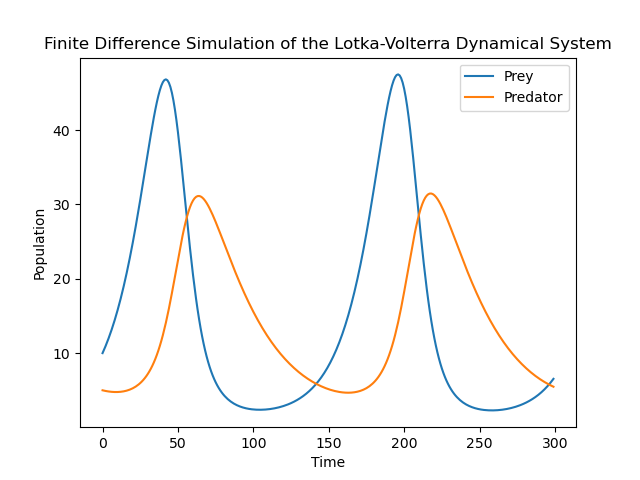
\includegraphics[width=0.75\textwidth]{Lotka-Volterra.png}
\caption{A simulation of the Lotka-Volterra equations using a finite-difference solution.}
\label{fig:LV}
\end{figure}
Before presenting the SSA implementation and the results, it is worth noting that the SSA algorithm is not likely to be accurate for problems involving small populations. This is because as the population decreases, the discrete decrement of the algorithm may result in completely extinct species, while as apparent in the solution shown in Fig. 1, neither species goes extinct, although their populations can become very low. To circumvent this situation, we apply the SSA algorithm to a transformed, but mathematically equivalent to the original, system of Lotka-Volterra equations. Specifically, we transform the original system into one of the type:
\begin{align}
\frac{dX'}{dt'} &= \alpha' X' - \beta' X'Y' \\
\frac{dY'}{dt'} &= \delta' X'Y' - \gamma' Y'
\label{eq:LV2}
\end{align}
where $X'$ and $Y'$ are scaled up populations of the prey and predator, and $\alpha'$, $\beta'$, $\delta'$, and $\gamma'$ are the associated rate constants of the system.  That is $X'=X \cdot s_f$ and $Y'=Y \cdot s_f$, where $s_f$ is a scaling factor.  We use $s_f=100$.  To make the system equivalent to the original, we need to set $\alpha'=\alpha/s_f$, $\beta'=\beta/s_f^2$, $\delta'=\delta/s_f^2$, $\gamma'=\gamma/s_f$, and $t'=t\cdot s_f$. Another observation is that a pray-predator interaction event has different impacts on the pray and predator populations. Therefore, we use $\beta' \cdot X' \cdot Y'$ as propensity function in the system and update the system using $X'=X'-1$ and $Y'=Y'+\frac {\delta} {\beta}$ to make the transitions consistent with the original system of equations.  The SSA algorithm is implemented in the following Python code:

\begin{lstlisting}[language=Python]

def get_tau_and_transition(X,Y,alpha,beta,gamma):
    tot_prop=alpha*X/s_f+beta*X*Y/s_f**2+gamma*Y/s_f
    r=np.random.rand()
    tau=-np.log(r)/tot_prop
    r=np.random.rand()
    if r<alpha*X/s_f/tot_prop:
        return 1,tau
    elif r<(alpha*X/s_f+beta*X*Y/s_f**2)/tot_prop:
        return 2,tau
    else:
        return 3,tau
    
def update_state(X,Y,alpha,beta,gamma,delta):
    r,tau=get_tau_and_transition(X,Y,alpha,beta,gamma)
    if r==1:
        return max(2,X+1),max(2,Y),tau
    elif r==2:
        return max(2,X-1),Y+1*delta/beta,tau
    else:
        return X,max(2,Y-1),tau
\end{lstlisting}

The outcome of a simulation using the SSA is shown in Fig. 2. As apparent, the SSA simulation is in good agreement with that produced by the finite-difference solution. Nevertheless, it should be mentioned that the SSA algorithm is computationally more expensive than the finite-difference solution, and is not the best option for problems that do not involve conservation of populations or mass. Specifically, the SSA simulation may drift away from true solution of the system without any objective to determine whether a drift occurred. In systems involving conservation of populations or mass, drifts cannot occur as the number of individuals or their mass is preserved.  In such cases, the SSA algorithm may be a better option than numerical deterministic solutions, especially if the interactions among species are complex and involve some randomness. An example of such a system is the stochastic coalescence of cloud droplets, Gillespie \cite{Gillespie1975}. This is a system of equations that describes the time evolution of the number of cloud droplets of different sizes. The system is a good candidate for the SSA algorithm because the total mass is conserved, i.e. two cloud droplets of mass $m_i$ and $m_j$ can coalesce to form a cloud droplet of size $m_i+m_j$. Deterministic solutions of the system are possible but complicated as they involve the discretization of the mass of the cloud droplets in a large number of bins and then accounting for the interactions among the bins.  The complication stems in the fact that the truncation errors may lead to unphysical solutions (e.g. negative mass in some bins). Moreover, additional processes such as a fragmentation of cloud droplets, which are not easy to model deterministically, can be easily incorporated in the SSA algorithm.

\section{Conclusions}
In this note, we described the Master Equation associated with some types of ODEs and a Stochastic Simulation Algorithm to solve them. We provided a simple but intuitive proof of why the Master Equation and the ODE are equivalent, and why the associated probabilistic solutions work. We also provided a simple example of a population dynamics system of ODEs, and solved it using the SSA.

\begin{figure}
\centering
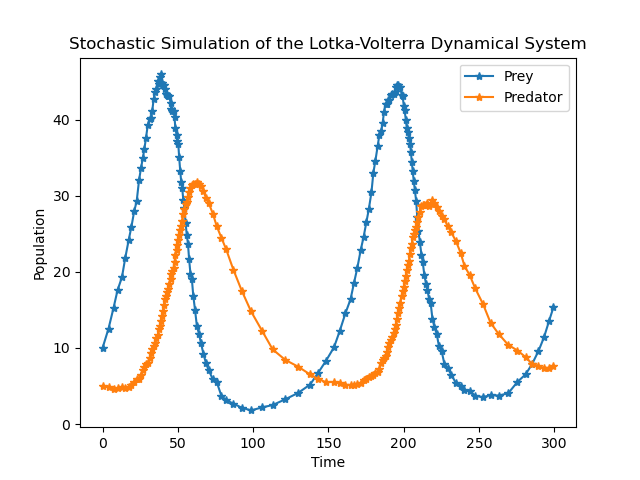
\includegraphics[width=0.75\textwidth]{Lotka-Volterra_SSA.png}
\caption{A simulation of the Lotka-Volterra equations using the SSA algorithm.}
\label{fig:LV_SSA}
\end{figure}
%% end document
%% add references
\begin{thebibliography}{9}
\bibitem{Gillespie1977}
Gillespie, D. T. (1977). Exact stochastic simulation of coupled chemical reactions. The Journal of Physical Chemistry, 81(25), 2340-2361.
\bibitem{introProb2005}
Dekking FM, Kraaikamp C, Lopuhaä HP, Meester LE. A Modern Introduction to Probability and Statistics: Understanding why and how. London: springer; 2005.
\bibitem{Gillespie2007}
Gillespie DT. Stochastic simulation of chemical kinetics. Annu. Rev. Phys. Chem.. 2007 May 5;58:35-55.
\bibitem{Gillespie1975}
Gillespie, D. T., 1975: An Exact Method for Numerically Simulating the Stochastic Coalescence Process in a Cloud. J. Atmos. Sci., 32, 1977\-1989, https://doi.org/10.1175/1520-0469(1975)032.
\end{thebibliography}
\end{document}